\section{Type checker}
The type checker implements the semantic rules of Ezuino specified in chapter \ref{semantics}. \\
We split the type checker into two visitors TypeCheckerVisitor and ReturnStatementVisitor. TypeCheckerVisitor checks that the condition in a boolean statement has the correct type and that expressions are legal. ReturnStatementVisitor ensures that the actual returned value of a program matches the type defined in the function declaration.
The way TypeCheckerVisitor type checks expressions is through a setup where every expression node extends that inherits from an interface called ITypeNode. The ITypeNode interface requires that every child class have the method for getting and setting a type attribute. When type checking happens, we then compare each node through the checkType method.
\begin{figure}[H]
\centering
\frame{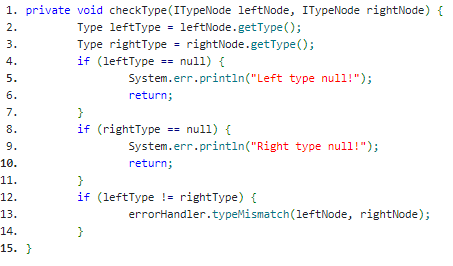
\includegraphics[scale=1.0]{figures/implementation/typeCecker/5-check-type.png}}
\caption{}
\label{dadsa}
\end{figure}

The boolean condition is checked in an if- and else statements.
 \begin{figure}[H]
\centering
\frame{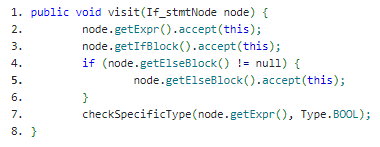
\includegraphics[scale=1.0]{figures/implementation/typeCecker/2-if-stmt.png}}
\caption{}
\label{lf05}
\end{figure}

An example of typechecking expressions. When an additive expression is reached both nodes are type checked.
\begin{figure}[H]
\centering
\frame{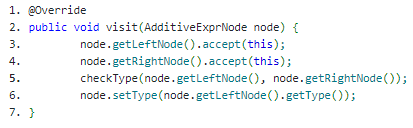
\includegraphics[scale=1.0]{figures/implementation/typeCecker/4-additive-typecheck.png}}
\caption{}
\label{lf05}
\end{figure}

In a unaryexpression it is also necessary to check that the operations performed are done with legal types. This is done through an switch case so it is easy to extend if more unary expressions needs to be added in the future. 
\begin{figure}[H]
\centering
\frame{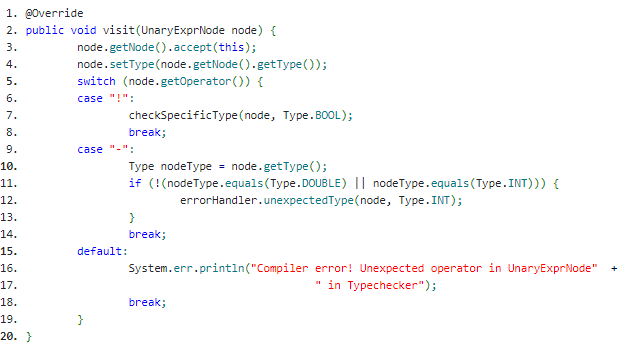
\includegraphics[scale=1.0]{figures/implementation/typeCecker/6-unary-expr.png}}
\caption{}
\label{lf05}
\end{figure}

When a return statement is returned it is set to its expression, this is important for type checking the return statement with the function declaration later in ReturnStatementVisitor.
It is also here that return in void functions is implemented. If a return statement has no value,we assume it to be a void function. This in practice makes the return key-word a way to preemptively end void functions.
\begin{figure}[H]
\centering
\frame{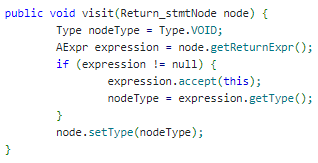
\includegraphics[scale=1.0]{figures/implementation/typeCecker/1-return-type.png}}
\caption{}
\label{lf05}
\end{figure}
This is the ReturnSatementVisitor. When a function is declared the type, it was declared as is temporarily saved in a symbol table. When a return statement is reached, the return statements type is compared with a type of the last function that was declared which was saved in the symbol table within that scope. This ensures that if there are several nested function declarations, the return type is compared to the most recent “active” scope.
\begin{figure}[H]
\centering
\frame{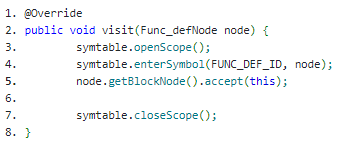
\includegraphics[scale=1.0]{figures/implementation/typeCecker/2-1-func-def.png}}
\caption{}
\label{lf05}
\end{figure}
 \begin{figure}[H]
\centering
\frame{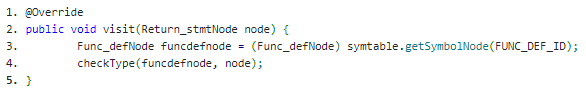
\includegraphics[scale=1.0]{figures/implementation/typeCecker/2-2-return-type-check.png}}
\caption{}
\label{lf05}
\end{figure}


\section{Checking that return are guaranteed}
If an function is not a void function, it should only be legal if it is guaranteed that it will reach an return statement. This means that if there is no return statement in the scope of the definition body, it must be because there is an if- and else block in the scope of the body where every if statement and the else statement have an return statement. 

\begin{figure}[H]
\centering
\frame{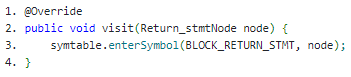
\includegraphics[scale=1.0]{figures/implementation/typeCecker/3-3-return-stmt-enter-symbol-table.png}}
\caption{If a return statement is encountered it, it is noted for the current scope.}
\label{lf05}
\end{figure}

\begin{figure}[H]
\centering
\frame{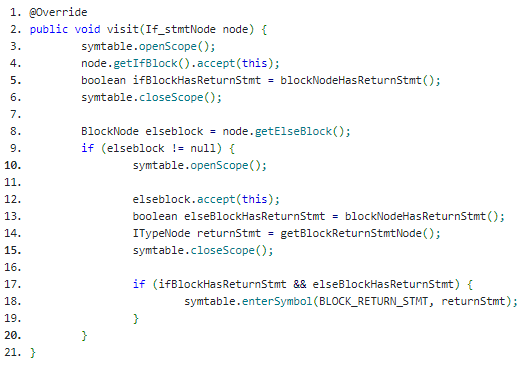
\includegraphics[scale=1.0]{figures/implementation/typeCecker/3-2-ifstmt-return-check.png}}
\caption{If an return statement in an if else block is guaranteed, it is noted for the current scope.} 
\label{lf05}
\end{figure}

 \begin{figure}[H]
\centering
\frame{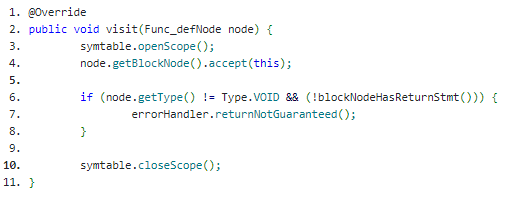
\includegraphics[scale=1.0]{figures/implementation/typeCecker/3-1-func-def-missing-return.png}}
\caption{If there is no return statement in the current scope, or an if else block where return is guaranteed throw an error.}
\label{lf05}
\end{figure}



\subsection{Func Structure Visitor (forstår den ikke helt, venter med den)}